In this section, we will formally define VTSs as a labeled graph
and the conditions on the graphs that are discussed in the previous
section.
%
Subsequently, we will present the SAT encoding of the search problems
for the graphs that satisfies the conditions.

\subsection{Model}

We model VTSs as labeled directed graphs.
The graph labels both nodes and edges with sets of molecules to denote
the set of molecules present in them.
The graph is formally defined as follows.

\begin{df}
  A VTS $G$ is tuple $(\nodes,\mols,\edges,\nlabel,\pairs,\edgef,\nodef)$, where
  \begin{itemize}
  \item $\nodes$ is a set of nodes representing compartments in the VTS,
  \item $\mols$ is the set of molecules flowing in the system, 
  \item $\nlabel : \nodes \maps \powerset{\mols}$ defines the molecules present in the nodes  
  \item $ \nodes \times (\powerset{\mols}-\emptyset) \times \nodes \subseteq \edges$ is the
    set of edges with molecule sets as labels
  \item $\pairs : \mols \times \mols$ is pairing relation
  \item $\nodef : \mols \maps \powerset{\mols} \maps \booleans$ is activity maps for nodes
  \item $\edgef : \mols \maps \powerset{\mols} \maps \booleans $ is activity maps for edges
  \end{itemize}
\end{df}
$\pairs$ defines which molecules can fuse with which molecules.
%
Let $\pairs(M')$ denote $\{m|(m,m') \in P \text{ and } m' \in M'\}$.
%
$\nodef$ and $\edgef$ are used to define activity of molecules on
nodes and edges respectively.
%
A molecule $k$ is {\em active} at node $n$ if $k \in \nlabel(n)$ and
$\nodef(k,\nlabel(n))$ is true.
%
A molecule $k$ is {\em active} at edges $(n,M',n')$ if $k \in M'$ and
$\edgef(k,M')$ is true.
%
We call $G$ {\em well-structured} if molecules $M$ is divided into
two equal partitions $M_1$ and $M_2$ such that $P \subseteq M_1 \times M_2$, and
for each $(n,M',n') \in \edges$, $n \neq n'$, 
$M' \subseteq \nlabel(n)$, and $M' \subseteq \nlabel(n')$.
%

We will also consider several variations of the model.
%
For example, unique edge between two nodes, activity of molecules is
not constrained by $\nodef$ and $\edgef$, etc.
%

A {\em path} in $G$ is a sequence $n_1,...,n_\ell$ of nodes 
such that $(n_i,\_,n_{i+1}) \in \edges$ for each $ 0 < i < \ell$.
%
For a molecule $m \in M$,
an {\em $m$-path} in $G$ is a sequence $n_1,...,n_\ell$ of nodes 
such that $(n_i,M',n_{i+1}) \in \edges$ and $m \in M'$ for
each $ 0 < i < \ell$.
%
A node $n'$ is {\em reachable} from node $n$ in $G$ if there is a path
$n,...,n'$ in $G$.
%
A node $n'$ is {\em $m$-reachable} from node $n$ in $G$ if there is a
$m$-path $n,...,n'$ in $G$.
%
We call $G$ {\em stable} if for each $(n,M',n') \in \edges$ and $m \in M'$,
$n$ is $m$-reachable from $n'$.
%
An edge $(n,M',n') \in \edges$ {\em fuses} with its destination node $n'$
if there are molecules $m,m' \in \mols$ such that $m$ is active in
$(n,M',n')$, $m'$ is active in $n'$, and $(m,m') \in \pairs$.
%
We call $G$ {\em well-fused} if each edge $(n,M',n') \in \edges$ fuses
with non-empty fusing molecules $M'' \subseteq M'$
and $\pairs(M'')$ are not active in any other node.



%
We call $G$ {\em connected} if for each $n,n' \in \nodes$,
$n'$ is reachable from $n$ in $G$.
%
We call $G$ $k$-connected if for each $\edges' \subseteq \edges$ and $|\edges'| < k$,
VTS $(\nodes,\mols,\edges-E',\nlabel,\pairs,\edgef,\nodef)$ is connected.


\paragraph{Search problem}
Based upon earlier discussion, we need to answer the following search
question among VTSs.
For a given $k$, size $\nu$, and molecule number $\mu$,
we are searching for well-structured, stable, and well-fused VTS
$G = (\nodes,\mols,\edges,\nlabel,\pairs,\edgef,\nodef)$ such that
$|\nodes| = \nu$, $|\mols = \mu|$, and
$G$ is not $k$-connected.    


\subsection{Boolean satisfiability of the search problem}

We translate the search problem into a Boolean satisfiability
problem and use SAT solvers to find the satisfying VTSs.
%
We will first present the variables used to encode the
VTSs and the properties.
%
Afterwards, we will present the formulas corresponding to the
properties.

\subsubsection{Variables for VTS description}
%
We assume that size of the graph is $\nu$ and number of molecules is
$\mu$.
%
Furthermore, we also limit the maximum number $\pi$ of edges present
between two nodes.
%
Here, we list the vector of Boolean variables and uninterpreted function symbols
that encode the VTSs.
\begin{enumerate}

\item Boolean variable $n_{i,m}$ indicates if $m \in \nlabel(i)$
\item Boolean variable $e_{i,j,q}$ indicates if $q$th edge exists between $i$ and $j$.
\item Boolean variable $e_{i,j,q,m}$ indicates if $q$th edge between $i$ and $j$ contains molecule $m$.

\item Boolean variable $p_{k,k'}$ indicates if $(m,m') \in \pairs$
\item uninterpreted Boolean functions $\nodef_m : \booleans^\mu \maps \booleans$
encoding $\nodef(m)$ map
\item uninterpreted Boolean functions $\edgef_m : \booleans^\mu \maps \booleans$
encoding $\edgef(m)$ map
\end{enumerate}
We also have auxiliary Boolean variables that will help us encode the well-fused and stability properties 
\begin{enumerate}
\item $a_{i,m}$ indicates that molecule $m$ is active at node $i$, i.e., $\nodef(m,L(i))$
  holds
\item $b_{i,j,q,m}$ indicates that molecule $m$ is active at $q$th edge $(i,M',j)$ between $i$ and $j$, i.e., $\edgef(m,M')$ holds
\item $r_{i,j,m,p}$ indicates that there is a path from $i$ to $j$ of length less than or equal to $p$
\end{enumerate}
For $k$-connected property, we also use the following auxiliary Boolean variables
\begin{enumerate}
\item $d_{i,j,q}$ indicates $q$th edge between $i$ and $j$ is dropped
\item $r'_{i,j}$ indicates that there is a path from $i$ to $j$ is a modified VTS
\end{enumerate}

We will describe the Boolean formulas that encode VTSs in several categories.
%
In the end, we will present in a table the formulas needed for the
model variants.
%
To avoid cumbersome notation, we will not explicitly write the ranges of the indexing
in the formulas.
%
$i$ and $j$ will be ranged over nodes.
%
$m$ will be ranged over molecules.
%
$q$ will be ranged over edges between two nodes.
%

% \subsubsection{Constraints on the structure of the edges, nodes and }
\subsubsection{Constraints on presence, activity of the molecule, and pairing matrix}
%
We need the following constraints~\eqref{eq:f0} and~\eqref{eq:c3}
to encode the basic structure of VTSs.
%
For an edge to exist it should have one molecule present. 
%
\begin{align}
  \bigwedge\limits_{i,j,q} (\bigvee_m e_{i,j,q,m} )\limplies e_{i,j,q}\tag{V1}\label{eq:f0}
\end{align}
If a molecule is active on an edge, it should be present on the edge.
%
\begin{align}
  \bigwedge\limits_{i,j,q,m} b_{i,j,q,m} \limplies e_{i,j,q,m}\tag{V2}\label{eq:f1}
\end{align}

A molecule should be present to be active on a node.  
\begin{align}
  \bigwedge\limits_{i,m} a_{i,m} \limplies n_{i,m}
  \tag{V3}\label{eq:c4}
\end{align}

The edge labels are subset of the node label of source and target compartments.

\begin{align}
  \bigwedge\limits_{i,j,q,m} e_{i,j,q,m} \limplies n_{i,m}\tag{V4}\label{eq:c0}\\
  \bigwedge\limits_{i,j,q,m}  e_{i,j,q,m} \limplies n_{j,m}\tag{V5}\label{eq:c1}
\end{align}

%C1 =  e_ijk -> aik and e_ijk -> ajk

Self edges are not allowed. 

\begin{align}
   \bigwedge\limits_{i,q} \neg e_{i,i,q}\tag{V6}\label{eq:c2}
\end{align}

Since a molecule cannot be both SNARE and tether,
we set diagonal blocks in pairing matrix to be 0's.
It reduces the search space.
% Condition on $p_{kk'}$. \ashu{why???} .
\begin{align}
  \bigwedge\limits_{(x < M/2 \, \land  \, y < M/2) \lor  (x >= M/2 \land y >= M/2)} \neg p(x,y)
  \tag{V7}\label{eq:c3}
\end{align}

\subsubsection{Well-fused constraints}
Boolean constraint~\eqref{eq:fuse1} encodes that each edge must fuse with
its destination node.
%
Boolean constraint~\eqref{eq:fuse2} encodes that each edge should not
be able to potentially fuse with any node other than its destination node.
\begin{align}
  \bigwedge\limits_{i,j,q} e_{i,j,q} \limplies \bigvee_{m,m^{\prime}} (b_{i,j,q,m} \land a_{j,m^{\prime}} \land p_{m,m^{\prime}})
  \tag{V8}\label{eq:fuse1}  \\
\bigwedge\limits_{i,j,q,m} b_{i,j,q,m} \limplies \neg \bigvee_{j \neq j^{\prime}, m^{\prime\prime}} ( a_{j^{\prime},m^{\prime\prime}} \land p_{m,m^{\prime\prime}})
  \tag{V9}\label{eq:fuse2}  
\end{align}


% Fusion rules consist of two different mechanisms.
% \begin{enumerate}
% \item  A \textbf{pairing mechanism} which determines compatible Q-R pairs on vesicles and compartments that can cause fusion.
% \item \textbf{regulatory mechanisms} on the edges and nodes (possibly distinct) which regulates molecules activity based on the presence/absence of other molecules on the corresponding node or edge.
% \end{enumerate}
% Boolean constraint~\eqref{eq:fuse1} and~\eqref{eq:fuse2} are used to encode well-fused
% property.

% F4: For an edge to be valid, at least one SNARE pair on the vesicle and target compartment must be active and have a non-zero entry in the pairing matrix.  

% F5: To ensure that fusion respects the graph structure by the edge under consideration, it should not be possible to fuse with any other node.


\subsubsection{Regulation on nodes and edges}
We are considering several models that differ in constraints on
the activity of molecules.
%
We will present~\eqref{eq:ann}-~\eqref{eq:aep} that encodes
the varying constraints.
%
The following formula encodes no conditions on activities on nodes,
i.e., all the present molecules on the nodes are active.
\begin{align}
\bigwedge\limits_{i,m} n_{i,m} = a_{i,m}    \tag{Ann}\label{eq:ann}
\end{align}
The following formula encodes that activity of a molecule $m$ on the node is
defined by a Boolean function $\nodef_m$ of presence of molecules present on that node.
\begin{align}
\bigwedge\limits_{i,m} n_{i,m} \limplies a_{i,m} =  \nodef_m (n_{i,1},\dots,n_{i,\mu}) 
\tag{Anb}\label{eq:anb}
\end{align}
The following formula encodes no conditions on activities on edges,
i.e., all the present molecules on the edges are active.
\begin{align}
  \bigwedge\limits_{i,j,q,m} e_{i,j,q,m} = b_{i,j,q,m}
\tag{Aen}\label{eq:aen}
\end{align}
The following formula encodes that activity of a molecule $m$ on the edge is
defined by a Boolean function $\edgef_m$ of presence of molecules present on that edge.
\begin{align}
   \bigwedge\limits_{i,j,q,m} e_{i,j,q,m} \limplies b_{i,j,q,m} = \edgef_k(e_{i,j,q,1}, .., e_{i,j,q,\mu} )
  \tag{Aeb}\label{eq:aeb}
\end{align}
%
The following formula encodes that the activity of the molecules on
edges is defined by inhibition by other molecules based on the pairing
matrix. 
\begin{align}
   \bigwedge\limits_{i,j,q, m}  [e_{i,j,q,m} \limplies  \bigwedge_{m' \neq m} (p_{m,m'} \limplies e_{i,j,q,m'})] \lequiv (\neg b_{i,j,q,m} \land  \bigwedge_{m' \neq m, p_{m,m'}} \neg b_{i,j,q,m'})
  \tag{Aep}\label{eq:aep}
\end{align}
% \[ \bigwedge\limits_{i,j,q, k}  (e_{i,j,q,k} \land [ ( \bigvee_{k'} p_{k,k'} \land \bigwedge_{k' != k} p_{k,k'} \limplies e_{i,j,q,k'})] ) \limplies \neg b_{i,j,q,k}) \, \]  

% \[ \bigwedge\limits_{i,j, q, k}  (e_{i,j,q,k} \land \neg [ ( \bigvee_{k'} p_{k,k'} \land \bigwedge_{k' != k} p_{k,k'} \limplies e_{i,j,q,k'})] ) \limplies b_{i,j,q,k}) \, \]  


% - F0: b(i,j,k) $\limplies$ e(i,j,k)

\subsubsection{Constraints for stability condition}
%
We use $m$-reachability to encode the stability condition in VTSs.
%
The following formula recursively encodes that node $j$ is $m$-reachable from node $i$ in less than $p$ steps
if either there is a direct edge between $i$ and $j$ with $m$ present on the edge or there is a edge between $i^{\prime \prime}$ and
$(i \neq i^{\prime \prime})$ with $m$ present, and j is $m$-reachable from $i'$ in less than $p-1$ steps.
%
\begin{align}
  \bigwedge\limits_{i,j,m,p} r_{i,j,m,p} \limplies (\bigvee_{q} \, e_{i,j,q,m} \lor \bigvee_{i\neq i^{\prime}} ( \, \bigvee_{q} e_{i,i^{\prime},q,m}) \land r_{i^{\prime},j,m,p-1} )
  \tag{R1}\label{eq:reach1}
\end{align}
Now we can encode stability using the reachability variables.
and say if there is an $m$-edge between $i$ and $j$, there is
$m$-reachable path from $j$ to $i$.\ashu{disjunction needed??}
\begin{align}
 \bigwedge\limits_{i,j,m} (\bigvee_{q} e_{i,j,q,m}) \limplies (r_{j,i,m,0}  \lor r_{j,i,m,1} \lor ... \lor r_{j,i,m,p})  
  \tag{R2}\label{eq:reach2}
\end{align}

% Boolean variable
% F3 and F2 are used to model these constraints. 

% % \textbf {Reachability definition and stability condition.}
% We have encoded stable condition by using reachability definition. \newline

% F3: Stability condition. For every leaving molecule, the source node is reachable from the target node with that molecule present, in maximum p steps. 


% F2: Reachability definition. Node j is reachable from node i with kth molecule present in maximum p steps if either there is a direct edge between i-j with that molecule present or there is a direct edge between $i^{\prime \prime}$ $(i \neq i^{\prime \prime})$ and j with kth molecule present on that edge and $i^{\prime \prime}$ are reachable from i in p steps. 


\subsubsection{$k$-connectivity constraints}
To check whether $k$-connected is a necessary condition, we remove (drop) $k-1$ edges from the graph and if it
disconnects the graph, and we get an assignment. We have a graph that is not  $k$-connected.
The following formulas encode the relevant constraints for reachability in the modified VTS. 

The following formulas encode that only existing edges can be dropped
and exactly $k-1$ edges are dropped.
\begin{align}
  \bigwedge\limits_{i,j,q} d_{i,j,q} \limplies e_{i,j,q}  \tag{D1}\label{eq:drop1}\\
  \sum_{i,j,q} d_{i,j,q} = k-1
  \tag{D2}\label{eq:drop2}
\end{align}
We need to define reachability in the modified VTS, therefore we use
a new variable $r'_{i,j}$ to encode reachability from $i$ to $j$.
In the following formula, we encode $r'_{i,j}$ is true if there is an
edge $(i,\_,j)$ and it is not dropped, or there is a node
$i^{\prime}$ such that, there is an edge $(i,\_,i^{\prime})$ which is
not dropped and $r'_{i',j}$ is true.
\begin{align}
\bigwedge\limits_{i,j}  [\bigvee_{q} (e_{i,j,q} \land  \neg d_{i,j,q}) \lor  (\bigvee_{i' \neq i}  r^{\prime}_{i',j} \land  \bigvee_{q} (e_{i,i',q} \land \neg d_{i,i',q}) ] \limplies r^{\prime}_{i,j}  
  \tag{D3}\label{eq:drop3}
\end{align}
Since we are looking for a graph that is not $k$-connected,
the following formula encodes that there are nodes $i$ and $j$ such that
there is no path between them in the underlying undirected graph.
\begin{align}
   \bigvee\limits_{i,j} \neg (r^{\prime}_{i,j} \lor r^{\prime}_{j,i})
  \tag{D4}\label{eq:drop4}
\end{align}

The key improvement in our work over the earlier tool is the
encoding of reachability, which was done using enumeration of paths.
%
In the current work, we have encoded reachability in two different
ways in formulas~\eqref{eq:reach1} and~\eqref{eq:drop3}.
%
The reachability is recursively defined in~\eqref{eq:drop3} and has
trivial solution by making all $r'$s true.
%
However, the trivial solution is disallowed by formula~\eqref{eq:drop4} and we find
only the solutions that captures the evidence of unreachability.
%
On the other hand,
we have added length of paths in our reachability encoding in formula~\eqref{eq:reach1},
which needs relatively more auxiliary variables.
%
This is because formula~\eqref{eq:reach2} has only positive
occurrences of the reachability variables and circular dependencies in
the recursive definition of $r'$s in ~\eqref{eq:reach1} may result
in spurious satisfying assignments that do not encode reachability.
%
By adding the path length, we break the circular dependencies, the
formula remains polynomial in size, and satisfying assignments only
corresponds to correct reachability.

% We can go down or up using -C \_ option.  \newline 

\subsection{SAT problems for different variants}
%\ankit{Bring model variant table here}

We have encoded several versions of the models of vesicle traffic systems listed. Starting from most basic version (A) where every present molecule is considered to be active. Other cases includes different combinations of constraints on the activity on nodes and edges. Most general restriction is activity of the molecule is dependent on the other molecules presence on the node (a Boolean function of N-1 parameters) (B,C,D,F,G,H). In very special case (E,F,G,H) activity of the molecules on the edges is dictated by pairing matrix, we call this process ``pairing inhibition". 
%In this case if the corresponding pairing molecules present on the edge with the molecules , both the molecule and all corresponding molecules gets inhibited/become inactive.  

% DIVIDE INTO COLUMNS and TALK ABOUT A/1 or A/0.
%\todo{describe the variations}

\begin{enumerate}[label=\Alph*]
\item Every present molecule is considered to be active.
\item Activity of molecules on the nodes is based on Boolean function of presence of other molecules. 
\item Activity of molecules on the edges is based on Boolean function of presence of other molecules
\item Activity of molecules both on the edges and nodes is based on Boolean function of presence of other molecules.
\item Activity of molecules on the edges is driven by pairing inhibition.
\item Activity of molecules on the nodes is based on Boolean function of presence of other molecules and on edge by pairing inhibition.
\item Version F with additional constraint that every edge is distinct.
%\item Activity of molecules on the nodes is based on Boolean function of presence of other molecules and on edge by pairing inhibition with every edge is distinct.
%\item Activity of molecules on the nodes is based on Boolean function of presence of other moleculess and on edge by pairing inhibition with self-edges are allowed.
%\item Version F but self-edges are allowed.
\end{enumerate}

We have applied the tool for the above variations for searching the vesicle traffic systems that satisfies
their corresponding properties. 

\begin{figure}
\centering
\begin{minipage}{0.50\linewidth}
  \hspace{-4ex}
\begin{tikzpicture}
\matrix [matrix of math nodes,left delimiter=(,right delimiter=),row sep=0.16cm,column sep=0.1cm] (m) {
\times & \times & \times &\times&\times&\times & \times & \times\\
\times & \times & \times&\times&\times&\times& 1 &\times \\
\times & \times & \times&\times&\times&1&\times &\times\\
\times & \times & \times&\times & 1 & \times &\times & \times\\
 \times & \times & \times & \times & \times & \times & \times & \times\\
 \times & \times & \times &\times & \times & \times & \times & \times\\
 \times & \times & \times & \times & \times & \times & \times & \times\\
 \times & \times & \times & \times & \times & \times&\times & \times\\};

\draw[dashed] ($0.5*(m-1-4.north east)+0.5*(m-1-5.north west)$) --
     ($0.5*(m-8-5.south east)+0.5*(m-8-4.south west)$);

\draw[dashed] ($0.5*(m-4-1.south west)+0.5*(m-5-1.north west)$) --
 ($0.5*(m-4-8.south east)+0.5*(m-5-8.north east)$);

\node[above=4pt of m-1-1] (top-1) {$M_1$};
\node[above=4pt of m-1-2] (top-2) {$M_2$};
\node[above=4pt of m-1-3] (top-3) {$M_3$};
\node[above=4pt of m-1-4] (top-4) {$M_4$};
\node[above=4pt of m-1-5] (top-5) {$M_5$};
\node[above=4pt of m-1-6] (top-6) {$M_6$};
\node[above=4pt of m-1-7] (top-7) {$M_7$};
\node[above=4pt of m-1-8] (top-8) {$M_8$};

\node[left=12pt of m-1-1] (left-1) {$M_1$};
\node[left=12pt of m-2-1] (left-2) {$M_2$};
\node[left=12pt of m-3-1] (left-3) {$M_3$};
\node[left=12pt of m-4-1] (left-4) {$M_4$};
\node[left=12pt of m-5-1] (left-5) {$M_5$};
\node[left=12pt of m-6-1] (left-6) {$M_6$};
\node[left=12pt of m-7-1] (left-7) {$M_7$};
\node[left=12pt of m-8-1] (left-8) {$M_8$};


\node[rectangle,above delimiter=\{] (del-top-1) at ($0.5*(top-1.south) +0.5*(top-4.south)$) {\tikz{\path (top-1.south west) rectangle (top-4.north east);}};
\node[above=10pt] at (del-top-1.north) {$Q-Snares$};
\node[rectangle,above delimiter=\{] (del-top-2) at ($0.5*(top-5.south) +0.5*(top-8.south)$) {\tikz{\path (top-4.south west) rectangle (top-6.north east);}};
\node[above=10pt] at (del-top-2.north) {$R-Snares$};

\node[rectangle,left delimiter=\{] (del-left-1) at ($0.5*(left-1.east) +0.5*(left-4.east)$) {\tikz{\path (left-1.north east) rectangle (left-4.south west);}};
\node[left=15pt,rotate=90,xshift=9mm] at (del-left-1.west) {$Q-Snares$};
\node[rectangle,left delimiter=\{] (del-left-2) at ($0.5*(left-5.east) +0.5*(left-8.east)$) {\tikz{\path (left-5.north east) rectangle (left-8.south west);}};
\node[left=15pt,rotate=90,xshift=9mm] at (del-left-2.west) {$R-Snares$};

\begin{pgfonlayer}{myback}

\foreach \element in {m-1-7,m-3-8,m-5-1,m-5-2,m-5-3,m-5-4,m-6-1,m-6-2,m-6-3,m-6-4,m-7-1,m-7-2,m-7-3,m-7-4,m-8-1,m-8-2,m-8-3,m-8-4}{
\highlight[pink]{\element}{\element}
}
\foreach \element in {m-2-7,m-3-6,m-4-5}{
\fhighlight[blue!10]{\element}{\element}
}
\end{pgfonlayer}

\end{tikzpicture}  
\end{minipage}
\begin{minipage}{0.45\linewidth}

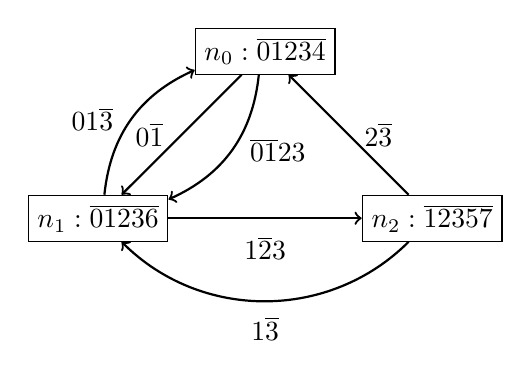
\begin{tikzpicture}[node distance = 30mm]
  \node[draw] (n0) {$n_0:\overline{01234}$};
  \node[draw,below left of=n0] (n1) {$n_1:\overline{01236}$};
  \node[draw,below right of=n0] (n2) {$n_2:\overline{12357}$};

  \draw[->,thick] (n0) -- node[left=1mm]  {$0\overline{1}$} (n1);
  \draw [->,thick] (n0) to [bend right=-30] node[right=1mm]  {$\overline{01}23$} (n1);
  \draw [->,thick] (n1) to [bend right=-30] node[left=1mm]  {$01\overline{3}$} (n0);

  \draw [->,thick] (n1) -- node[below=1mm]  {$1\overline{2}3$} (n2);
  \draw [->,thick] (n2) to [bend right=-45] node[below=2pt]  {$1\overline{3}$} (n1);

  \draw [->,thick] (n2) -- node[right=2pt]  {$2\overline{3}$} (n0);

\end{tikzpicture}
\end{minipage}

\caption{Pairing matrix} \label{fig:M1}
\end{figure}

%%% Local Variables:
%%% mode: latex
%%% TeX-master: "main"
%%% End:

\begin{figure}
\centering

\caption{Dia V2} \label{fig:v2}
\end{figure}


After creating the formula using different Boolean variables we ship them directly to the solver. In case of a satisfying (SAT) assignment of the added constraints the Z3 theorem prover gives a model with the variable assignment. In case no possible satisfying assignment the solver returns UNSAT.
%
%

% \subsection{Creating a solver and solving these constraints}
% We will create a solver and add these build formula using these constraints to that and then check whether there a satisfiable assignment that satisfies all these constraints.

% \begin{figure}[ht]
% %\vspace{-3mm}
% \begin{verbatim}
% # Create a solver
% s = Solver()
% # Add these formulas to it.
% s.add(A0, A1, C0, C1, C2, C4, C5, F0, F1, F2, F3, F4, F5, D0, D1, D2, D3)

% # Check for the satisfiability assignment.
% print s.check()   
% \end{verbatim}
% \caption{Solving for these constraints.}
% \label{code:motivate}
% \end{figure} 


%--------------------- DO NOT ERASE BELOW THIS LINE --------------------------

%%% Local Variables:
%%% mode: latex
%%% TeX-master: "main"
%%% End:
